\documentclass[12pt]{article}
\usepackage{rotating}
\usepackage{graphicx, subfigure}
\begin{document}

\section{Exploratory Data Analysis}

\begin{figure}[ht!]
     \begin{center}
        \subfigure[]{
            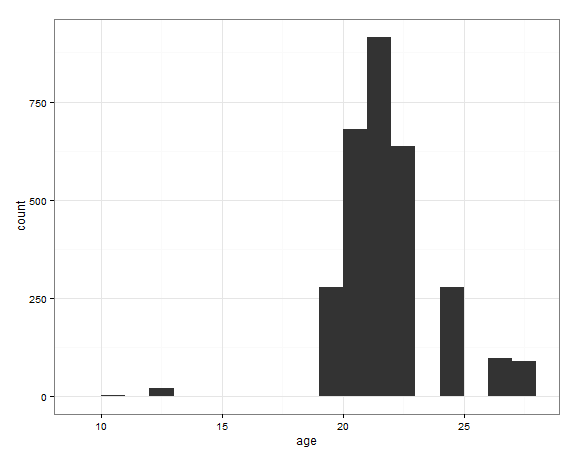
\includegraphics[width=0.45\textwidth]{../../output/demo_analysis/hist_age.png}
            \label{madison_results}
        }
        \subfigure[]{
           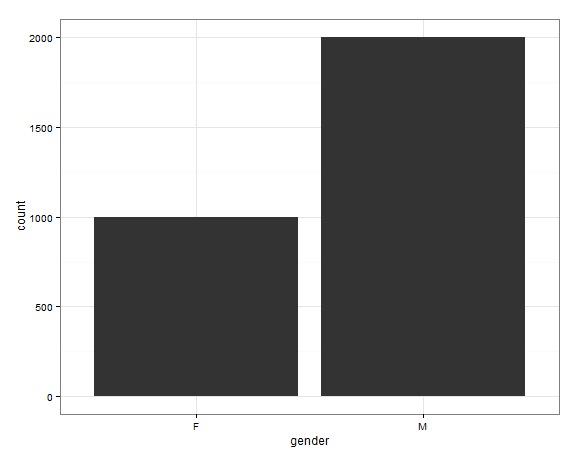
\includegraphics[width=0.45\textwidth]{../../output/demo_analysis/hist_gender.png}
           \label{phoenix_results}
		}
    \end{center}
    \caption{Histogram of age and gender of participants. }
\end{figure}

\begin{figure}[ht!]
     \begin{center}
        \subfigure[]{
            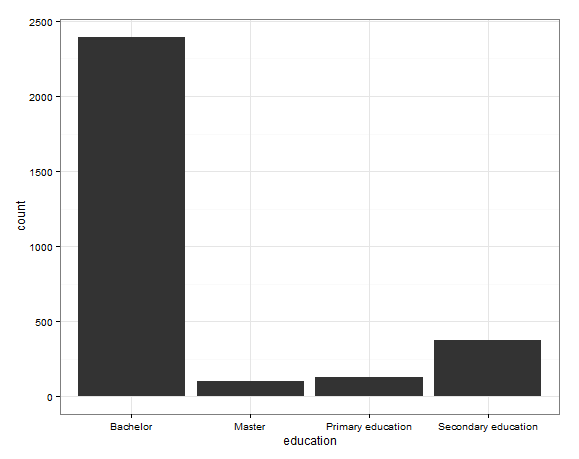
\includegraphics[width=0.45\textwidth]{../../output/demo_analysis/hist_edu.png}
            \label{madison_results}
        }
        \subfigure[]{
           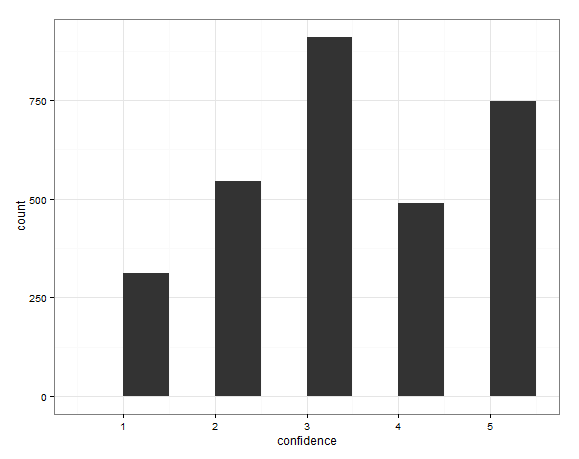
\includegraphics[width=0.45\textwidth]{../../output/demo_analysis/hist_confidence.png}
           \label{phoenix_results}
		}
    \end{center}
    \caption{Histogram of education level and confidence level. }
\end{figure}


\begin{figure}[ht!]
\begin{center}
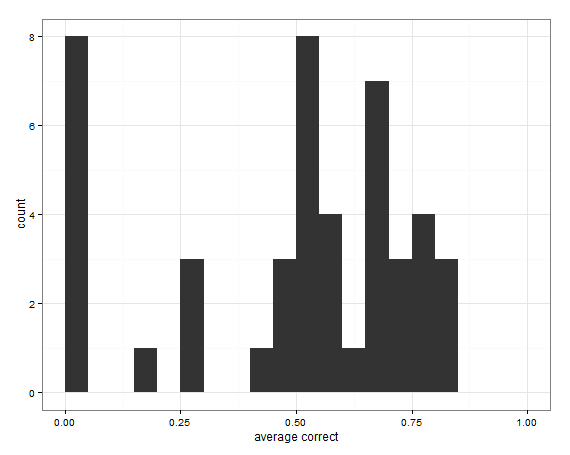
\includegraphics[width=0.45\textwidth]{../../output/demo_analysis/hist_user_perf_mc.png}
\caption{Histogram of user performance on multiple choice tasks.}
\end{center}	
\end{figure}


\begin{figure}[ht!]
     \begin{center}
        \subfigure[]{
            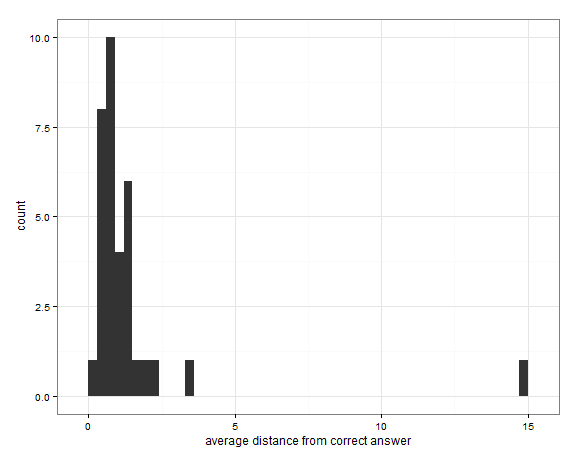
\includegraphics[width=0.45\textwidth]{../../output/demo_analysis/hist_user_perf_pe_tot.png}
        }
        \subfigure[]{
           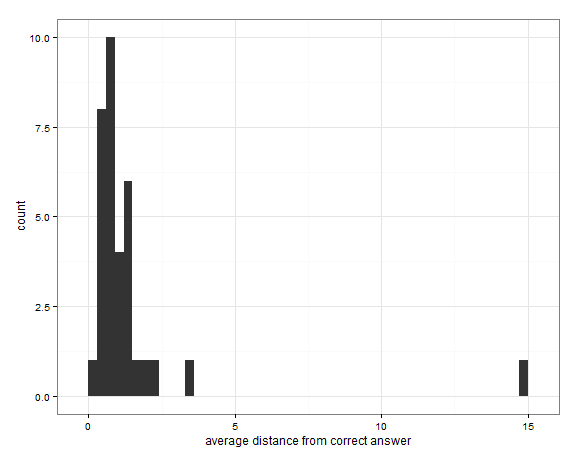
\includegraphics[width=0.45\textwidth]{../../output/demo_analysis/user_perf_pe_zoom.png}
		}
    \end{center}
    \caption{Histogram of aggregate user performance for point estimate tasks.}
\end{figure}

%\textsc{
%\begin{table}[ht!]
%\centering
%\begin{tabular}{rlr}
%  \hline
% & type & av\_score \\ 
%  \hline
%1 & audio & 0.10 \\ 
%  2 & image & 0.71 \\ 
%  3 & video & 0.65 \\ 
%   \hline
%\end{tabular}
%\caption{Average score by asset type for all domains.} 
%\end{table}

\begin{figure}[ht!]
\begin{center}
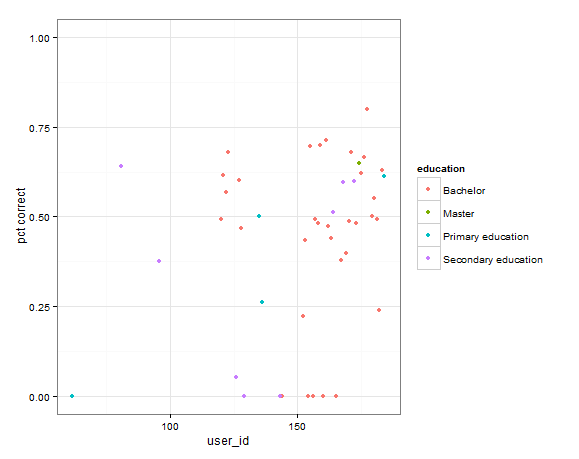
\includegraphics[width=0.45\textwidth]{../../output/demo_analysis/scatter_edu.png}
\caption{Scatter plot of accuracy by education level on multiple choice tasks.}
\end{center}	
\end{figure}


\begin{table}[ht!]
\centering
\begin{tabular}{rlrr}
  \hline
 & education & pct\_correct & av\_dist \\ 
  \hline
1 & Bachelor & 0.42 & 1.46 \\ 
  2 & Master & 0.52 & 1.28 \\ 
  3 & Primary education & 0.45 & 1.22 \\ 
  4 & Secondary education & 0.40 & 1.42 \\ 
   \hline
\end{tabular}
\caption{Average score by education level all domains.} 
\end{table}


\clearpage

\begin{table}[ht]
\centering
\begin{tabular}{rrrr}
  \hline
 & confidence & pct\_correct & av\_dist \\ 
  \hline
1 &   1 & 0.23 & 1.35 \\ 
  2 &   2 & 0.17 & 1.50 \\ 
  3 &   3 & 0.31 & 1.33 \\ 
  4 &   4 & 0.52 & 2.01 \\ 
  5 &   5 & 0.75 & 0.66 \\ 
   \hline
\end{tabular}
\caption{Average score by confidence level all domains.} 
\end{table}

\begin{figure}[ht!]
     \begin{center}
        \subfigure[]{
            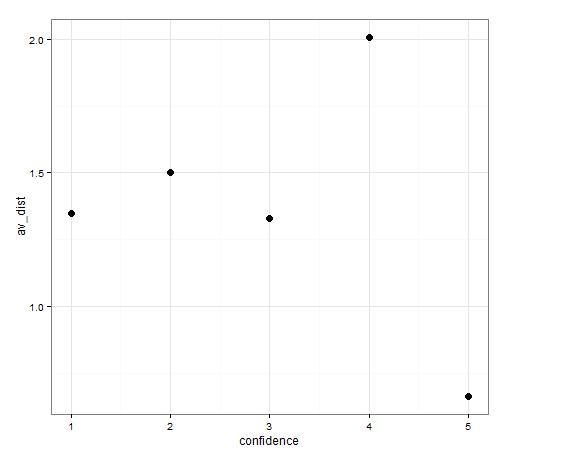
\includegraphics[width=0.45\textwidth]{../../output/demo_analysis/plot_conf_pe.png}
        }
        \subfigure[]{
           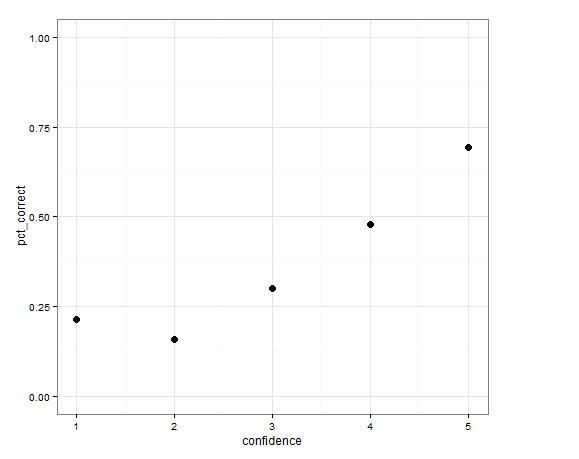
\includegraphics[width=0.45\textwidth]{../../output/demo_analysis/plot_conf_mc.png}
		}
    \end{center}
    \caption{Scatter plot of percent accuracy by reported confidence level for point estimate and multiple choice quesions. }
\end{figure}


\clearpage

\section{Crowd Rankings}

\begin{table}[ht!]
\centering
\begin{tabular}{rrlrr}
  \hline
 & domain\_id & domain\_name & crowd\_score & crowd\_rank \\ 
  \hline
   & 3 & MagicTrick & 20.00 & 1.00 \\ 
   & 7 & Landmarks & 18.00 & 0.92 \\ 
   & 12 & Penalties & 12.00 & 0.82 \\ 
   & 53 & MovieSong & 13.00 & 1.00 \\ 
   \hline
\end{tabular}
\caption{Multiple Choice domains. The Crowd Ranking column contains the percentage of users the crowd performs better than. Score is the number of answers the crowd got right.} 
\end{table}


\begin{table}[ht!]
\centering
\begin{tabular}{rrrrrrl}
  \hline
  & domain & mean & median & geom.mean & trunc.mean & trunc.geom.mean \\ 
  \hline
 &  Calories & 0.45 & 0.68 & 0.63 & 0.58 &  0.78\\ 
   \hline
\end{tabular}
\caption{Point estimate rankings by domain according to average ranking. Columns represent the ranking by using the corresponding method of aggregation. Average ranking takes the mean of the crowd percentiles for each task.} 
\end{table}



\end{document}